
%(BEGIN_QUESTION)
% Copyright 2010, Tony R. Kuphaldt, released under the Creative Commons Attribution License (v 1.0)
% This means you may do almost anything with this work of mine, so long as you give me proper credit

Beregn følgende parametere i denne 3-leder RTD-kretsen, gitt RTD-temperatur på 174 $^{o}$F og $\alpha = 0.00385$ $\Omega$/$\Omega$/$^{o}$C:

$$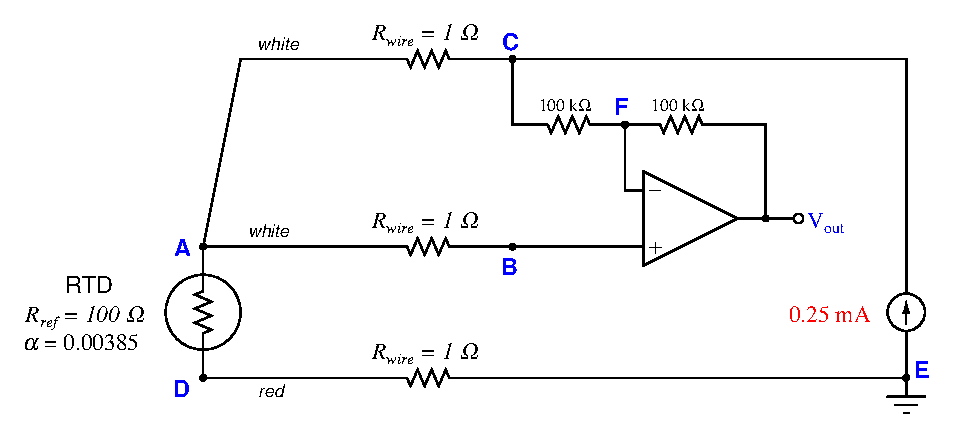
\includegraphics[width=15.5cm]{i00668x01.eps}$$

\begin{itemize}
\item{} $V_{out}$ = \underbar{\hskip 50pt} millivolt
\vskip 10pt
\item{} $V_{AD}$ = \underbar{\hskip 50pt} millivolt
\vskip 10pt
\item{} $V_{AB}$ = \underbar{\hskip 50pt} millivolt
\vskip 10pt
\item{} $V_{CB}$ = \underbar{\hskip 50pt} millivolt
\vskip 10pt
\item{} $V_{CF}$ = \underbar{\hskip 50pt} millivolt
\end{itemize}

Merk: Oppgi bare spenningsstørrelser, ikke polariteter, i svarene dine.

\underbar{file i00668no}
%(END_QUESTION)





%(BEGIN_ANSWER)

\begin{itemize}
\item{} $V_{out}$ = {\bf 32.59} millivolt (formel) \hskip 30pt {\bf 32.6175} millivolt (tabell)
\vskip 10pt
\item{} $V_{AD}$ = {\bf 32.59} millivolt \hskip 30pt {\bf 32.6175} millivolt (tabell)
\vskip 10pt
\item{} $V_{AB}$ = {\bf 0} millivolt
\vskip 10pt
\item{} $V_{CB}$ = {\bf 0.25} millivolt
\vskip 10pt
\item{} $V_{CF}$ = {\bf 0.25} millivolt
\end{itemize}

%(END_ANSWER)





%(BEGIN_NOTES)

{\bf Denne oppgaven er ment for eksamen, ikke arbeidsark.}

%(END_NOTES)
